\subsection{Description of the data model}

This section describes the data model used in Obvious and the way to create data structures. It also exposes the util package for the data model.  The data model used in Obvious has been largely specified during the workshop: a consensus has been found among all participants.

\begin{figure}[!h]
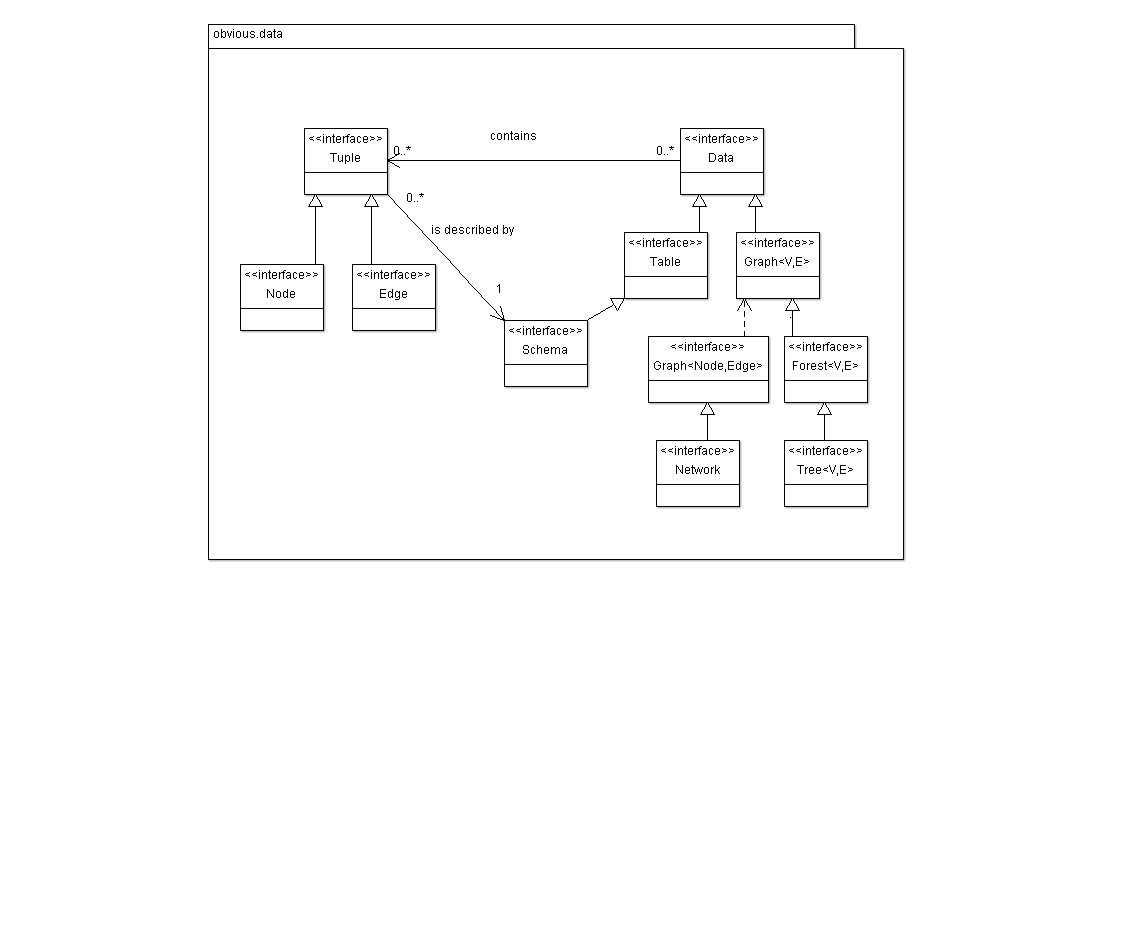
\includegraphics[width=\columnwidth]{figures/obviousdataclass}
\caption{Class diagram of the data model}
\label{fig:datamodel}
\end{figure}

The initial data model proposed for Obvious derived from the proxy tuple design pattern exposed in \cite{DesignPatternsIV}. Obvious adopts this design pattern since Obvious wants to offer for the data model high extendability and good usability. Among all the patterns introduced in \cite{DesignPatternsIV}, the proxy tuple pattern proposes both points since it describes graphs in an object-oriented manner - many developers are used to manipulation of \emph{object oriented graphs} - and since it unifies the data model around the same standard structure (tuples and tables).

In our data model, tuples are standards elements of all structures: tables are composed of tuples and graphs/trees are implemented as networks i.e. graphs built around two tables one for the nodes and the other for the edges. Nevertheless, a major difference exists between our pattern and those introduced in \cite{DesignPatternsIV}. Our data model used schema to describe the columns of a table (their type, name and default value) instead of a column object, that does not exist in Obvious. Schemas have been introduced, since they are efficient to gather all \emph{meta-data} for the columns of a table in one unique structure, allowing easy table and network instantiations with a factory.

Thus, this model is completed by factories, that allows data structure instantiations. Logically, they used the well known factory pattern. With those factories, it is possible to instantiate tables and networks from a schema or from an existing object from a targeted Obvious implementation (e.g. a Prefuse table or a JUNG graph...). This also provides the possibility to use parameters to provide more arguments used in targeted toolkits. For example, in the Prefuse implementationof Obvious, parameters are used to specify the source and target node columns for a graph in an edge table.

Finally, we have defined an utility package obviousx, named in the same way as javax. This package provides different kinds of utility classes for the Obvious data model. First, we have defined in obviousx, reader and writer interfaces allowing the creation of gateways between the Obvious data model and common data formats such as CSV and GraphML. It is useful since it gives software developers a standard way to import and export data in Obvious whatever the underlying implementation of the data model is. In addition, for data providers, it simplifies their work because they only have to develop one reader and one writer to be compatible with a large number of toolkits. With the same logic, obviousx furnishes a Java TableModel compatible with the Obvious one: it allows quick creation of a JTable from an Obvious
table. Finally, obviousx also provides wrappers to \emph{transform} obvious data structures into common existing data structures (Prefuse, Ivtk, Jung, more to develop) in order to avoid copying of data when using more than one data model.
 
\subsection{Notification system}

Information visualization toolkits (such as other softwares) uses notification systems to propagate information about changes affecting the data model. During the development of Obvious implementations, notification systems included in toolkits appears to be widely different in terms of syntax and functionalities. That is why the notification system introduced in Obvious is designed to support a large variety of existing notification techniques even those not currently implemented in toolkits. For example, it supports transaction and batch techniques usually found in database system.

As in many toolkits \cite{Prefuse,InfoVis,jung2003}, the notification system in Obvious is based on listeners placed on data structures that propagates changes to listening objects. Since one operation can affect a large amout of data, flow of notifications concerning the same action could be generated. Thus, we introduce a method to control the number of emitted notifications: the \emph{beginEdit/endEdit mechanism}. The way this mechanism acts can differ from one implementation to another: no notification emitted when the mechanism is triggered or it can start a transaction.
